As part of the C3Pro Project, a framework has been developed in JAVA to test the elaborated change negotiation and propagation algorithms for collaborative processes. The framework already provides functions for importing process models in form of BPMN 2.0 XML. Within this importing process, the BPMN models are converted into a framework internal graph representation without loosing any information about the control flow and connection objects of the original model. This resulting graph structure then enables modest model manipulation and analysis techniques.\par
In order to save the effort of implementing the same or at least a likewise graph model structure for the automatic process collaboration generator, it was decided to integrate it into the existing framework. Hence, the structure and it's complementary components and services can be utilized with minor adoptions.\par
The following chapters describe the internal process model representation structure, the algorithms and components of the implemented automatic generator as well as the translation algorithm to transfer the resulting models to BPMN 2.0 XML.

\section{Internal Process Model Representation}
The framework internal process model representation utilizes the jBPT\footnote{Business Process Technologies for Java - https://code.google.com/p/jbpt/} library, which was developed by Polyvyanyy et. al \cite{jbpt} in the context of their compendium of process technologies and facilitates the development of process models in JAVA. Figure \ref{fig:jbpt} shows an excerpt of the core structure of the library. The structure enables the creation of different types of graphs to support the capturing of various process modeling languages, such as petri nets, EPC\footnote{Event-driven process chains} or BPMN.\par
For the purpose of constructing BPMN process models, an implementation of the \textit{AbstractMultiDirectedGraph} class is suitable. A \textit{multi directed graph} represents a graph, whose vertices can be connected among themselves through more than one \textit{directed} edges\cite{graph_theory}. Figure \ref{fig:jbpt} also shows that all graph models are typed with generics. In the context of a \textit{multi directed graph} model, the parameter \textit{E} is bound to a an instance of \textit{IDirectedEdge\textless$V$\textgreater}, whereas parameter \textit{V} is bound to an instance of \textit{IVertex}. 

\begin{figure}[H]
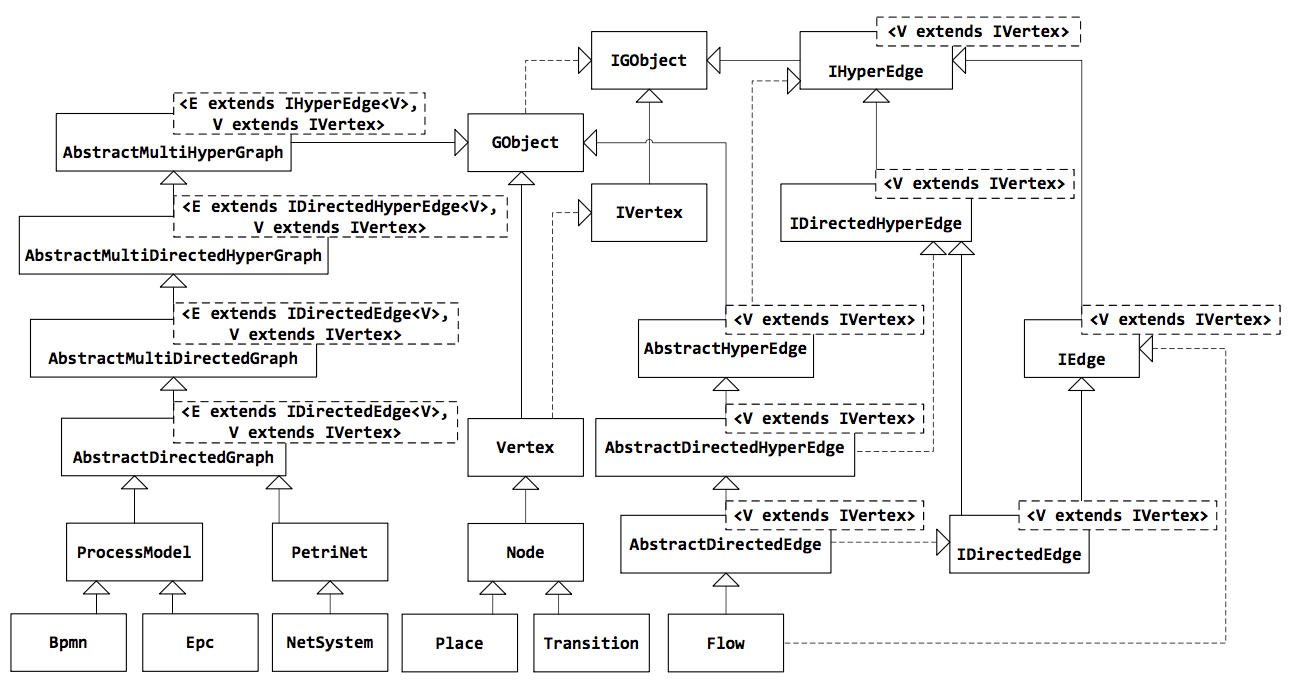
\includegraphics[width=1\textwidth]{src/images/class_diagram_jbpt.png}
\caption{Class and interface hierarchy of jBPT}
\label{fig:jbpt}
\end{figure}

In order to utilize the jBPT structure to build any type of BPMN process model, all specific BPMN flow objects, must therefor implement the \textit{IVertex} interface. The flow objects, for instance tasks or gateways, are then in turn connected through Edges, which represent the BPMN sequence flow, to create the graph and therefor the process model. How the jBPT library is incorporated and utilized by the C3Pro framework is illustrated in figure \ref{fig:choreo_structure}. 
The intensive use of interfaces, enables the reuse of flow objects, that are part of different model types. For instance, gateways and events are used in all four. For the sake of clarity, figure \ref{fig:choreo_structure} only shows model specific flow objects, that are appropriate for BPMN choreography models. Table \ref{tab:flow_objects} lists all BPMN flow objects, that are supported by the C3Pro framework to create process collaborations and their different models.\\

\begin{table}[H]
\resizebox{\textwidth}{!}
{
\begin{tabular}{l|cccc}
			      & Choreography Model & Collaboration Model & Public Model & Private Model \\ \hline
Start Event       & $\blacksquare$	  & $\blacksquare$      & $\blacksquare$	  & $\blacksquare$  \\
End Event         & $\blacksquare$	  & $\blacksquare$      & $\blacksquare$	  & $\blacksquare$  \\
Parallel Gateway  & $\blacksquare$    & $\blacksquare$      & $\blacksquare$      & $\blacksquare$  \\
Exclusive Gateway & $\blacksquare$    & $\blacksquare$      & $\blacksquare$      & $\blacksquare$  \\
Interaction       & $\blacksquare$    & $\square$           & $\square$           & $\square$       \\
Task          	  & $\square$         & $\blacksquare$      & $\blacksquare$      & $\blacksquare$  \\
Send Task         & $\square$         & $\blacksquare$      & $\blacksquare$      & $\blacksquare$  \\
Receive Task      & $\square$         & $\blacksquare$		& $\blacksquare$      & $\blacksquare$       
\end{tabular}%
}
\caption{Overview of supported BPMN flow objects}
\label{tab:flow_objects}
\end{table}

Within the C3Pro framework, all four model types support the flow objects \textit{start event, end event, parallel gateway} and \textit{exclusive gateway}. These are basic control flow objects, that are not specific to any model type in BPMN. Additionally available, for \textit{collaboration, public} and \textit{private models} are the activities \textit{Task, Send Task} and \textit{Receive Task}. According to the BPMN 2.0 specification, the activity \textit{task} represents an \textit{abstract task} \cite{BPMN20}. An \textit{abstract task} is a task that is not further specified. There are several further specified tasks in BPMN, including the also supported \textit{send} and \textit{receive task}. Since the focus of the C3Pro project is on collaborative processes and the message exchange between the participating partners, it's mandatory that these two messaging activities are also specified within the framework. For the remaining activities, that are not part of the message flow, it is in this context not relevant if the task is actually a \textit{user, manual, service} or \textit{script task}. The only flow object specific for \textit{Choreography Models} is the \textit{Choreography Task} or \textit{Interaction}, the equivalent of a \textit{send} and \textit{receive task} sequence in a collaboration model.   

\begin{figure}[H]
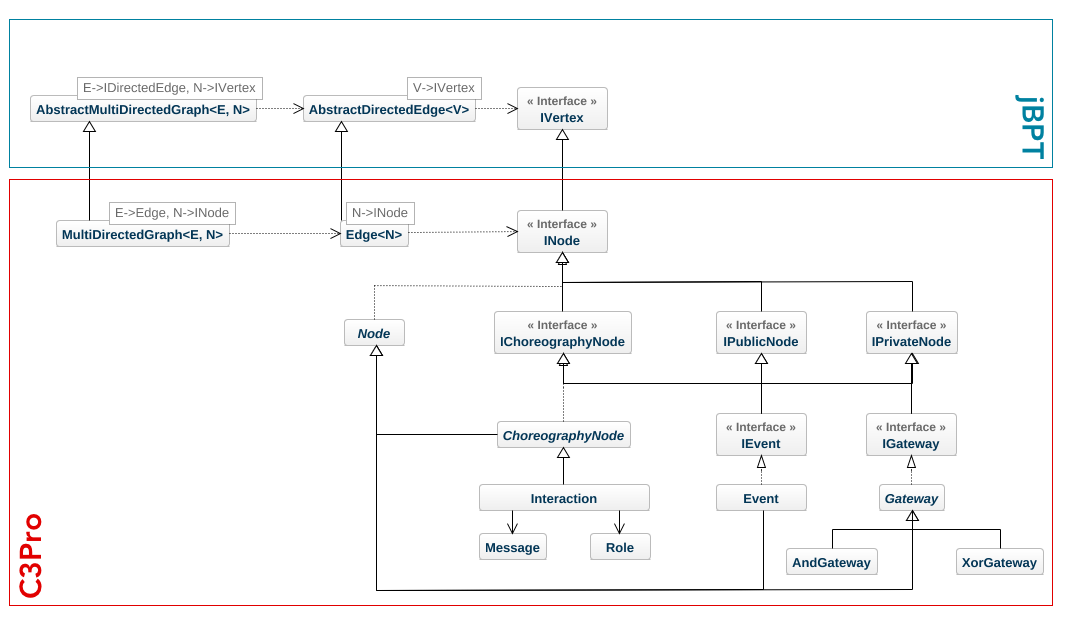
\includegraphics[width=1\textwidth]{src/images/c3pro_graph_structure.png}
\caption{C3Pro Model Representation Structure}
\label{fig:choreo_structure}
\end{figure}

\section{Approach}

As already mentioned in the chapter of theoretical background, a process collaboration between several partners can be modeled from different perspectives (partner or global) through the use of different model types. The process collaboration generator implemented in the context of this work, generates all four different model types as the outcome. In general, there exist two different approaches to build a process collaboration with all the described models \cite{sabrina1174}. At the \textit{top-down approach}, first the choreography model is build. Based on the choreography, then the public and private models of each partner are defined consistently. On the other hand, at the \textit{bottom-up approach}, each partner has already defined a private and public process. Then, the choreography model is constructed by connecting the public models via message exchange. \par
The automatic generator, presented in this work, follows the \textit{top-down approach}, by first generating the choreography model and then deriving the collaboration, public and private models from it. Thereby, each interaction (choreography task) of the choreography model, is converted into an send and receive task and then added to the involved partners processes, to build their public process models. Then in turn, each private model is derived from it's corresponding public model by enriching the public model with some abstract private tasks. The collaboration model is then build by compositing the partner's public processes into one model.\\

Generally, when defining business process models, three levels of correctness that build upon each other must to be considered and satisfied by the models: \\

\begin{wrapfigure}{r}{0.5\textwidth}
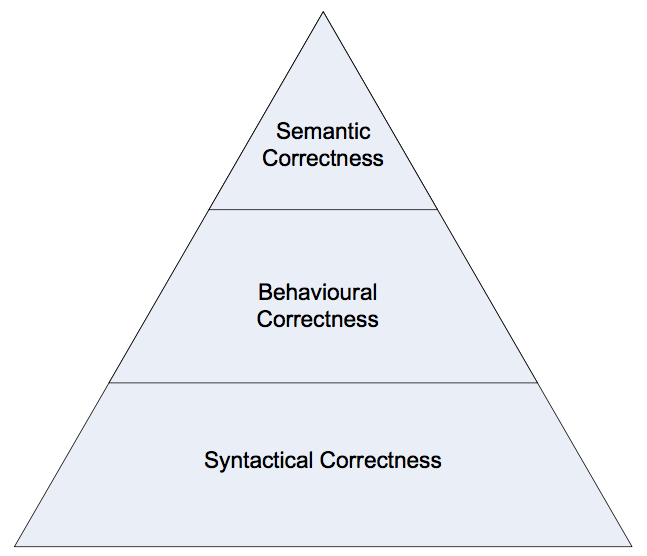
\includegraphics[width=0.9\linewidth]{src/images/correctness_levels.png}
\caption{Pyramid of Business Process Model Correctness}
\label{fig:bpm_correctness}
\end{wrapfigure}

\textit{Syntactical Correctness} is defined by the underlying BPMN meta model and refers to the correct use and composition of the corresponding model elements. Syntactical constraints for example include, that any model must have at least one start and one end event, as well as that flow objects (e.g. tasks, gateways, events) can only be connected by control flow edges \cite{sabrina848}. \\

\textit{Behavioral Correctness} constitutes that a process model must be executable and therefor to be free of deadlocks or lifelocks. It presumes that the model is syntactical correct, because the behavior of a syntactical incorrect model is undefined. Regarding collaborative, cross-organizational processes, it is also required that the composition of the involved public models are compatible. For example, this means, that for every message that is send, a corresponding partner must be able to receive it \cite{sabrina1174, sabrina848}. \\

\textit{Semantic Correctness} means that the a process model must comply with imposed compliance rules \cite{sabrina848}. Thereby it must be differentiated between \textit{local} and \textit{global compliance rules}. \textit{Local compliance rules} constrain the private process of a partners, whereas \textit{global compliance rules} constrain the interaction between multiple partners \cite{sabrina1174}. In this work, only \textit{global compliance rules} are imposed to constrain the choreography model. \\

All three levels of correctness are considered by the developed algorithm of the implemented automatic process generator. The algorithm ensures that only model specific flow objects are used to build the processes and that they are connected appropriately (syntactical correctness). It also guarantees the absence of deadlock and lifelocks (behavioral correctness) and offers the possibility to define global compliance rules (see next chapter), to which the generated collaboration complies to (semantic correctness). The introduced approach of deriving all models out of the before generated choreography model offers also the advantage, that if the deriving process is implemented correctly, it already ensures \textit{consistency} and \textit{compatibility} between the different models. In the context of collaborative processes, \textit{consistency} means, that the private model of a partner has to be consistent with the corresponding public model. This ensures that the executed business process of one partner satisfies the behavior that is communicated to the partners through his public models \cite{sabrina1174}. \\

\section{Constraining the Collaboration Generation}

Despite the premise, that the process collaborations should be generated randomly, it is reasonable to set some boundaries within the random generation takes place. The implemented generator provides two different ways to influence the resulting choreography model and hence the whole collaboration. The first one, provides the possibility to constrain the choreography model in terms of the employed flow objects and their exact quantity by specifying several input parameters. The second one, let the user impose global compliance rules based on compliance patterns to which the resulting model must comply to.

\subsection{Parametric Constraints} \label{sec:param_constraints}

Following input parameters are specified to influence the random generation of the choreography model and hence also the deriving models:

\begin{itemize}
\item Number of Partners
\item Number of Interactions
\item Number of Exclusive Gateways
\item Number of Parallel Gateways
\item Number of Loops
\item Max. Branching
\end{itemize}

\textit{Number of Partners} determines the number of participants which are involved in the process collaboration, whereas \textit{Number of Interactions} specifies the number of messages which are exchanged between the partners. \textit{Number of Exlusive/Parallel Gateways} in combination with \textit{Max. Branching} influences the the branching of the resulting process model. The First applies the exact number of the respective flow object into the model, whereas the second sets the upper boundary of branching (splitting the path) for each gateway. The lower boundary is set to two. Within this range, the generating algorithm determines a random number of following paths for each gateway placed into the model. This is explained in more detail later one. \textit{Number of Loops} determines the exact number of loops that should be placed into the model.

\subsection{Compliance Constraints}

Generally, compliance rules can be defined for different process flow perspectives of a process. It can be distinguished between compliance rules that constrain the control flow (sequence of activities), the data associated with the activities, the resources (specific user or role) that perform the activities or the time perspective. There exist several languages and approaches on how to define and specify compliance rules, including formal languages \cite{Ghose2007},\cite{GovMilSad:edoc:06:compliance}, visual languages \cite{sabrina953},\cite{Awad2008} and pattern-based approaches \cite{compliance_patterns}, \cite{Ramezani2012}. Both, visual and pattern-based approaches, aim at hiding formal details (e.g. temporal logic) and therefore simplifying the specification of compliance rules. \\

For the specification of compliance rules for the automatic process generator, the pattern-based approach of Turetken et. al. \cite{compliance_patterns} is utilized. In \cite{compliance_patterns} a repository of \textit{process control patterns} is introduced, which are high-level templates used to represent process properties which the process specification must satisfy. There are four different groups of patterns: 

\begin{itemize}
\item \textit{Order} patterns concern the sequencing of activities. For Instance, `\textit{Customer\_Inquiry} LeadsTo \textit{Offer}', is used to express that after a inquiry is send and received, an offer must be prepared and send.
\item \textit{Occurrence} patterns represent rules to address the existence of certain activities. For instance, `\textit{Check\_Credit\_Worthiness} Universal', is used to express that the activity must always occur when the process is executed. 
\item \textit{Resource} patterns constrain that certain activities must be performed by a specific user or group of users (role). For instance, `\textit{Approve\_Offer} PerformedBy \textit{Role Q}' constrains, that the activity must be assigned to a user who is part of the user group Q.    
\item \textit{Time} patterns are used to assign temporal rules to Order or Occurrence patterns. For instance, `\textit{Customer\_Inquiry} LeadsTo \textit{Offer} Within \textit{7(days)}' constrains, that an Offer has to be replied within seven days after an inquiry has been received. 
\end{itemize}

Because the generated process collaborations neglects the data, time and resource perspective and focuses solely on the control flow, only compliance rules that constrain the sequence of activities are possible to impose. Following process control patterns are supported to constrain the automatic generated choreography:

\begin{table}[H]
\centering
\resizebox{12cm}{!}
{
\begin{tabular}{l|l}
Pattern		      & Description  \\ \hline
P LeadsTo Q       & Interaction P must lead to Interaction Q	  	 \\
P Precedes Q      & Interaction Q must be preceded by Interaction P	  \\
P Universal  	  & Interaction P must always occur throughout execution \\
P Exists		  & Interaction P must be specified in process \\
\end{tabular}%
}
\caption{Overview of supported Compliance Patterns}
\label{tab:compl_patterns}
\end{table}



\section{Random Collaboration Generation Process}

The class diagram shown in figure \ref{fig:choreo_gen_structure} gives a simplified overview of all the components which are necessary for generating an entire process collaboration, starting with the generation of the choreography model to imposing compliance rules and finishing with deriving the public and private models. It also shows the major operations provided by every component. 

\begin{figure}[H]
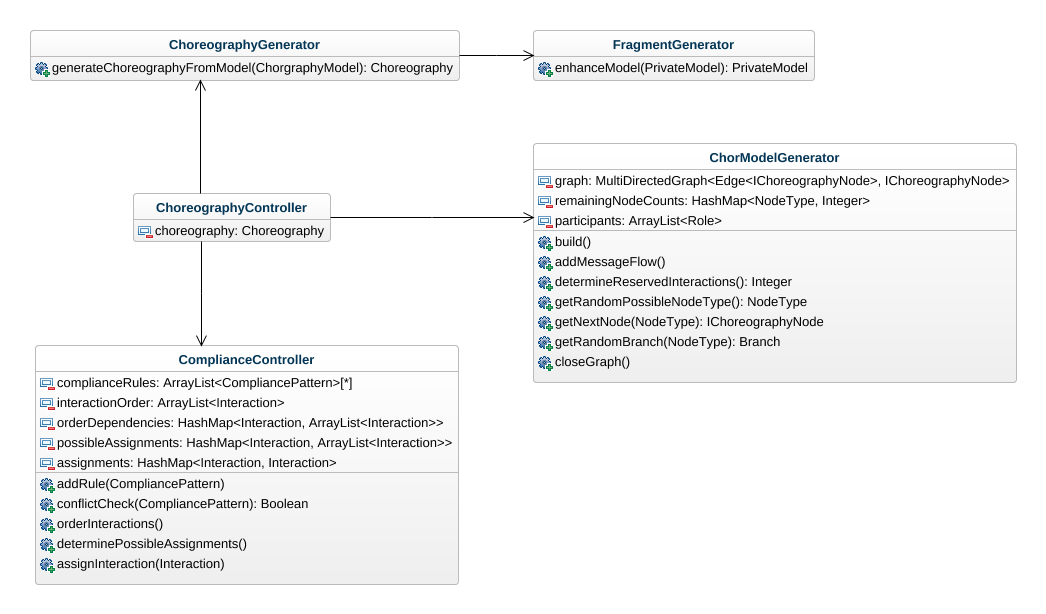
\includegraphics[width=1\textwidth]{src/images/ChorGen_Class.png}
\caption{Class Structure Choreography Model Generator}
\label{fig:choreo_gen_structure}
\end{figure}

In the following the components and their functionalities will be explained in detail.

\subsection{Choreography Controller}
The \textit{ChoreographyController} class represents the orchestration component for building random process collaborations, based on given constraints. The process follows the principle \textit{'first build then check'}, which means that after a random model has been generated, it will then be checked if the interactions defined within the compliance rules, can be assigned into the already built model in such a way that the resulting interaction sequence complies to the imposed rules. If the interaction allocation is not possible without violating the compliance rules, new random models will be build until a compliant model has been generated. Thereby the number of interactions will be increased by 10 percent every 10th build. After the successful assignment of the compliance rules, the remaining public and private models will be derived out of the generated choreography model. At last all models will be exported to a valid BMPN XML file. The whole process of generating a random choreography by coordinating the different functions is outlined with Algorithm \ref{alg:choreographyController}. \\

\begin{algorithm}[H]
\SetAlgoLined
\KwData{}
\KwResult{}
buildSuccess = \textbf{false}\;
\While{buildSuccess $\neq$ \textbf{true}}{
	build new choreography model\;
	\eIf{compliance rules are defined}{
		assign interactions\;
		\uIf{assignment successful}{
			buildSuccess = \textbf{true}\;
		}\ElseIf{number of interaction $\bmod$ 10 $\equiv$ 0}{
			increase number of interactions by factor 1.1\;
		}

	}{
		buildSuccess = \textbf{true}\;
	}
}
generate choreography\;
export models to BPMN\;
\caption{How to write algorithms}
\label{alg:choreographyController}
\end{algorithm}

\subsection{Choreography Model Generator}
The actual algorithm for generating graphs, representing choreography models, is implemented within the \textit{ChoreographyModelGenerator} component. Throughout the graph building process, it is essential to keep track of the current graph state at every point, in order to know where in the graph it is possible to put a new node without violating the syntactical correctness of the resulting BPMN model.  
Therefore a data model and corresponding logic is introduced in the \textit{GraphTracking} component, 
wherein the model is broken down into \textit{splits}, \textit{branches} and \textit{nodes}. A split is created for every gateway fork, that is put into the model. Every split has several branches (minimum two and maximum is defined by the max\_branching parameter), 
which are representing the different paths created by an parallel or exclusive gateway.    
Each branch holds the set of nodes that are on the path of this branch, whereas a path is limited by the merge node of it's corresponding fork gateway (split). In terms of a choreography model, nodes are limited to interactions and gateways.

\begin{figure}[H]
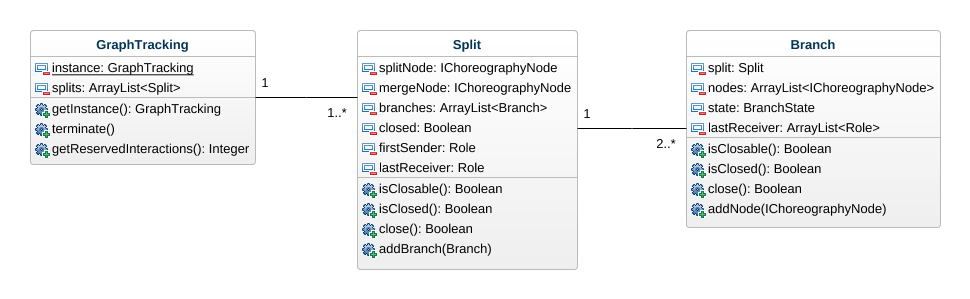
\includegraphics[width=1\textwidth]{src/images/graphtracking_cd.png}
\caption{Datamodel GraphTracking}
\label{fig:graphTracking2}
\end{figure}

Figure \ref{fig:graphTracking1} illustrates the concept of the \textit{GraphTracking} component. In this example, there are in total three splits with the split nodes: start event (blue), exclusive gateway\#1 (red) and parallel gateway \#1 (green). The split with the start event as the split node and the end event as the merge node has always only one branch, the main branch. Technically, this is not a split in the sense of the terminology. But because of the underlying data model, which is shown in figure \ref{fig:graphTracking2}, that defines that every branch must be related to a split, this pseudosplit is necessary to keep track of the main branch. The main branch (split \#1 - branch \#1) holds the set of ordered nodes: Interaction \#1, XOR gateway \#1, XOR merge \#1 and Interaction \#10.\\
Split \#2 has three branches. The first branch contains the nodes Interaction \#2 and Interaction \#5. The second branch consists only of Interaction \#3 and the third branch contains AND gateway \#1, AND merge \#1 and Interaction \#9. At last, the third split consists of two branches, which are holding the remaining interactions \#6, \#8 and \#7 respectively. 

\begin{figure}[H]
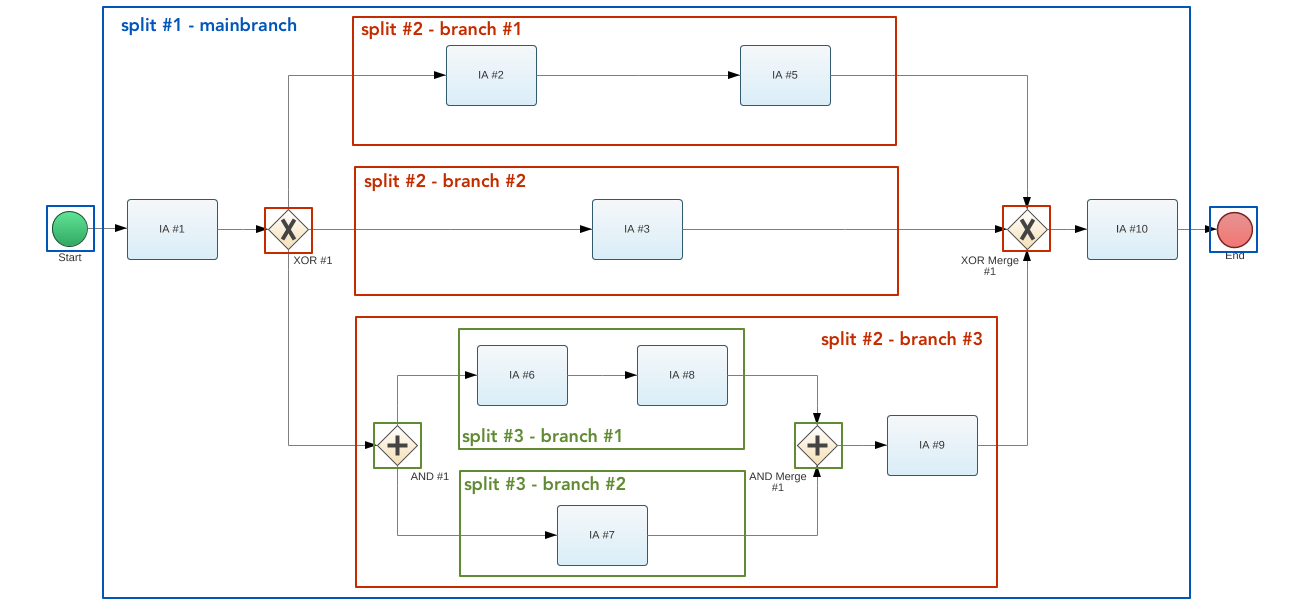
\includegraphics[width=1\textwidth]{src/images/graphTracking_1.png}
\caption{Concept of GraphTracking component}
\label{fig:graphTracking1}
\end{figure}

Furthermore, every split and every branch has a status. This status indicates whether the branch or split is \textit{open} or \textit{closed}. In case of a branch, open defines, that the branch is not yet enclosed by the merge node of it's corresponding split node and can further evolve by putting more nodes on its path. In turn, closed defines, that the branch is already finished by a connection of the last node with the respective merge node. A split is marked as closed, if all its branches are connected with the corresponding merge node, thus are closed. Additional to these two status, a branch can also be in the state \textit{split}. A branch has the state \textit{split}, if it contains a split and none of this split's branches are yet closed, thus there exists no merge node for this split. In this case, a branch can not evolve until one of it's enclosed branches is in state \textit{closed} and a merge node is placed on the split branch. Then the state changes from \textit{split} to \textit{open}. For example, in figure \ref{fig:graphTracking3}, the branch \#1 of split \#2 represents a branch in state \textit{split}, whereas the mainbranch is in state \textit{open} because branch \#2 of split \#1 is already closed by the merge node of split \#2.\\
During the build process it is also necessary to determine if a branch is allowed to be closed, without violating the soundness of BPMN choreography models. A branch is marked as closable, if there is an interaction on all it's enclosed paths. This approach of tracking the status of the branches becomes crucial the less remaining interactions are available and the more branches are still open in the model. Because of the parametric limitation of the number of interactions, at a certain point in the build process, not every open branch is allowed to be randomly selected for placing the next interaction or gateway without resulting in violating the correctness of the model or exceeding the number of interactions. In order to determine if this situation applies to a current point in a build process, the \textit{GraphTracking} component monitors the amount of \textit{free interactions} and \textit{reserved interactions}. 

\begin{figure}[H]
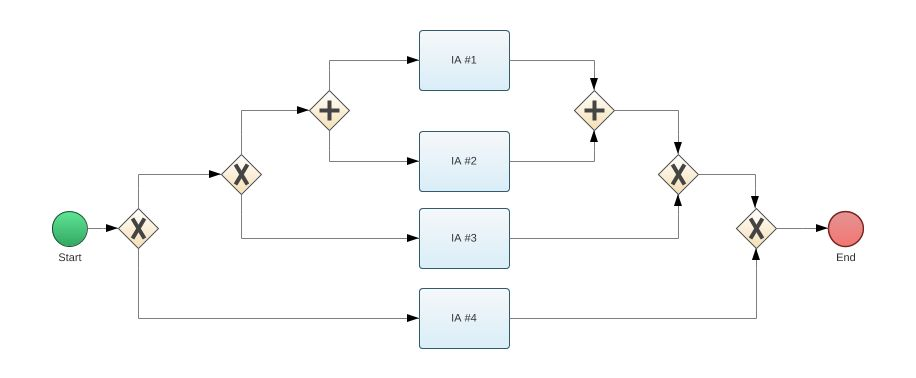
\includegraphics[width=1\textwidth]{src/images/proof_interactions.jpeg}
\caption{Minimum Interactions reserved by remaining gateways}
\label{fig:graphTracking4}
\end{figure}

Reserved interactions, are a certain amount of the remaining interaction that have either predetermined positions in the current graph (resInteractionsBranches) or will be needed in further paths created by not yet employed gateways (resInteractionsGateways). The exact amount of these reserved interactions, is depending on the number of not closable branches of the current graph and the number of gateways, that are not yet put into model. Regarding the current model, each open and non closable branch, increases the amount of \textit{resInteractionsBranches} by one. Gateways, that are not yet placed into the graph, will later create at least two new branches, that then again need at least one interaction on each of it's paths. Considering that a gateway node is allowed to be immediately followed by another gateways node without an interaction in between, the minimum amount of \textit{resInteractionsGateways} is $remaining gateways$ + 1. This influence of nested gateways onto the minimum amount of reserved interactions is illustrated in figure \ref{fig:graphTracking4}. After the amount of reserved interactions is calculated, the number of free interactions is determined by the difference between the amount of remaining interactions and the number of reserved interactions (see also definition \ref{def:def1}). If the amount of \textit{free interactions} $\equiv$ 0 then the random selection of the position in the graph is limited to the branches that are not yet closable, hence have not yet an interaction on their path. On the other hand, if the amount of \textit{free interactions} $\>$ 0, then all open branches can be selected for putting the next node.

\begin{Def}
	Let $x$ be the number of branches which are open and not closable, \\$remainingInteractions$ all the interactions not yet put into the model and \\$remainingSplits$ all the number of splits not yet put into the model. Then
	\begin{center}
		\textbf{resInteractionsBranches} = x\\
		\textbf{resInteractionsGateways} = $remainingSplits$ + 1\\
		\textbf{resInteractionsTotal} = $resInteractionsModel$ + $resInteractionsGateways$\\
		\textbf{freeInteractions} = $remainingInteractions$ - $reservedInteractionsTotal$
	\end{center}
	\label{def:def1}
\end{Def}


\begin{figure}[H]
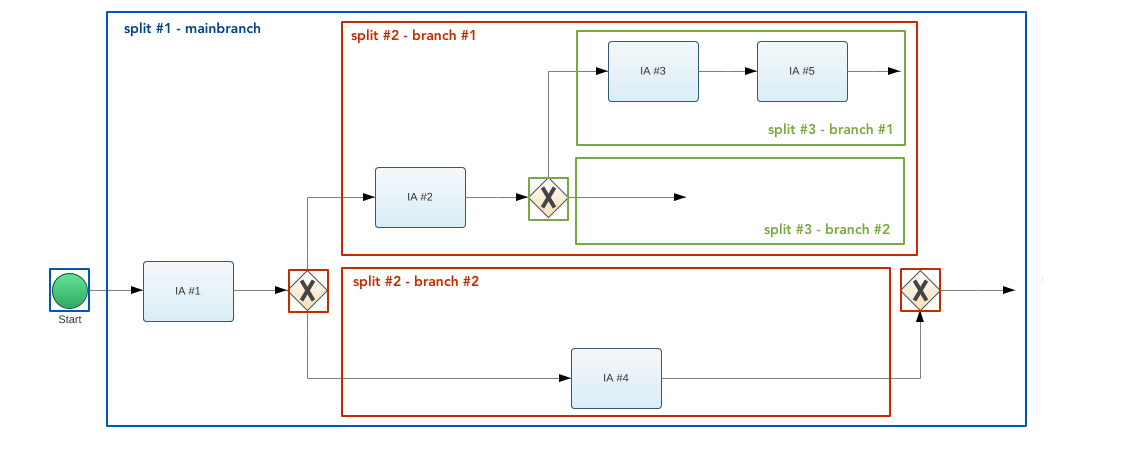
\includegraphics[width=1\textwidth]{src/images/graphTracking_status.png}
\caption{Minimum Interactions reserved by remaining gateways}
\label{fig:graphTracking3}
\end{figure}

Assuming a model generation where the total number of interactions being 6 and the total number of gateways being 2, the unfinished model in figure \ref{fig:graphTracking3} shows a choreography model at the point during the build process where not all open branches are allowed to be selected for placing the node (in this case an interaction). In order to obtain a sound choreography model while not increasing the number of initially specified interactions, the sixth interaction is only allowed to be placed on branch \#2 of split \#3. In this scenario, \textit{reservedInteractions} equals to one and \textit{freeInteractions} therefor equals to zero. On the other hand, if assuming the total number of interactions being 7, all branches of split \#3 and the mainbranch are possible candidates for placing the sixth interaction, because at this point, \textit{freeInteractions} would equal to one. \\

\begin{algorithm}[H]
\DontPrintSemicolon
\SetAlgoLined
\SetKwInOut{Input}{Input}\SetKwInOut{Output}{Output}
\Input{ 
\begin{itemize}[label={--}]
\setlength\itemsep{0em}
\item $remainingNodes \leftarrow$ number of nodes by type
\item $participants \leftarrow$ number of participants
\item $loops \leftarrow$ number of loops
\end{itemize}
}
\SetKwProg{Fn}{Function}{}{}
\SetKw{Continue}{continue}
\Begin{
	\If{number of interactions $\leq$ number of gateways + 1}{
		model generation is not possible\;
	}
	$graphTracking \leftarrow$ initialize GraphTracking\;
	\While{$remainingInteractions > 0$}{ 
		$nextNodeType \leftarrow$ getRandomNodeType()\;
		$selectedBranch \leftarrow$ getRandomBranch()\;
		\eIf{$selectedBranch$ is closable}{
			close branch by random\;
			\If{closed}{
				\Continue
			}
		}{
			$nextNode \leftarrow$ instantiate node of $nextNodeType$\;
			\If{$nextNodeType$ is gateway}{
				$branchCount \leftarrow$ getRandomBranchCount()\;
				$split \leftarrow$ instantiate new split\;
				$graphTracking.splits \leftarrow$ split\; 
				\For{$i \leftarrow$ 0 $branchCount$}{
					$branch \leftarrow$ instantiate new branch\;
					$split.branches \leftarrow branch$\;
					$i \leftarrow i$ + 1\;
				}
				add split and branches to SplitTracking\;
			}
			$selectedBranch.nodes \leftarrow$ $selectedBranch.nodes \cup nextNode$\;
			decrease $remainingNodes$ of $nextNodeType$\;
		}
	}
	close still open splits\;
	add end event to main branch\;
	enrich interactions with reasonable sender and receiver sequence\;
}
\caption{Generate Choreography Model}
\label{alg:choreoGen}
\end{algorithm}
\pagebreak
The actual procedure of generating random choreography models is shown in algorithm \ref{alg:choreoGen}. The input for a random model generation are the parametric constraints introduced in section \ref{sec:param_constraints}. At first, it is checked if the specified combination of the amount of interactions and gateways are sufficient to generate a sound model. This is the same evaluation as in determining the reserved interactions by remaining gateways. Therefore, the amount of interactions must be $\geq$ the amount of gateways + 1. If the validation is successful, the GraphTracking component gets instantiated. Thereby a split for the start event and the mainbranch is created. After GraphTracking is set up successfully, the algorithm loops over the number of remaining interactions until all interactions are put into the model. Within each loop, at first a node type for the next node is randomly selected out of the pool of remaining nodes. This can be an interaction, exclusive or parallel gateways depending on the number of free and reserved interactions. If there are free interactions available, the node type interaction is always in the pool of possible next node types. In case there are no free interactions left, the node type interaction will only get included in the possible next node types if not all remaining interactions are reserved by not yet consumed gateways. The algorithm for random possible node type selection is shown in \ref{alg:randNodeType}.\\

\begin{algorithm}[H]
\DontPrintSemicolon
\SetAlgoLined
\Begin{
	possibleNodeTypes $\leftarrow$ \{\}\;
	\If{freeInteractions $>$ 0 $\lor$ remInteractions $>$ resInteractionsGateways }{
		possibleNodeTypes $\leftarrow$ possibleNodeTypes $\cup$ Interaction\;
	}
	\If{remainingParallelGateways $>$ 0}{
		possibleNodeTypes $\leftarrow$ possibleNodeTypes $\cup$ ParallelGateways\;
	}
	\If{remainingExclusiveGateways $>$ 0}{
		possibleNodeTypes $\leftarrow$ possibleNodeTypes $\cup$ ExclusiveGateways\;
	}
	\Return random NodeType of possibleNodeTypes\;	
}
\caption{getRandomNodeType()}
\label{alg:randNodeType}
\end{algorithm}

After a node type has been selected, a position in the model is determined for placing a node of the previously selected node type by randomly selecting a possible open branch. Which branches are in the pool of possible, selectable branches, is again depending on whether there are free interactions available or not. If there are free interactions left, all open branches are allowed to be selected, independent from the prior selected node type. This changes if there are no free interactions remaining. In this case, only all open are allowed to be considered for random selection if again, not all remaining interactions are reserved by not yet consumed gateways. Otherwise only branches that are closable are allowed to be included in the pool of possible branches. The algorithm for random possible branch selection is shown in \ref{alg:randBranch}.\\

\begin{algorithm}[H]
\DontPrintSemicolon
\SetAlgoLined
\Begin{
	possibleBranches $\leftarrow$ \{\}\;
	\eIf{freeInteractions $>$ 0 $\lor$ remInteractions $>$ resInteractionsGateways }{
		possibleBranches $\leftarrow$ all open branches\;
	}{
		possibleBranches $\leftarrow$ all not closable branches\;
	}
	\Return random Branch of possibleBranches\;	
}
\caption{getRandomBranch()}
\label{alg:randBranch}
\end{algorithm}

In the next step, the random selected branch is checked whether it's closable or not and if so gets closed by random. This doesn't apply to the mainbranch to make sure that there is always one branch where the model can further evolve. This step of random branch closing is necessary to obtain balanced choreography models regarding nested branches. If there is no random branch closing mechanism the resulting models would be very similar. A mechanism that closes branches whenever they are possible to close would only result in models with lesser nested branches whereas a mechanism that never closes branches would result in models that have highly nested branches. If the selected branch gets randomly closed, a merge node for this branches split is created and added to the enclosing branch. Additionally, in the data model of the corresponding split, the merge node gets noted in order to assure that the last nodes of the other branches of this split will get connected with the same merge node when they get closed. Finally the algorithm jumps back to the beginning of the loop and starts again with randomly selecting a possible node type for the next node to be placed in the model.\\
By the time a branch is not randomly closed, a node of the predefined node type gets instantiated. In case of an interaction, only the plain object without any sender, receiver or message gets instantiated. Is the selected node type a gateway, the number of branches is determined by randomly selecting a number between 2 and the current maximum branching amount. The upper boarder of the maximum branching amount is generally limited by the user specified max branching parameter. But again, due to the limitation of interactions, the specified maximum amount of branches can not be adducted as the upper boarder without considering the current amount of free interactions. If only the user specified upper branching boarder is adducted, there is a high chance that this results in an inconsistent model, because there are not enough interactions for all paths that are created. In order to prevent this, the possible upper limit is determined dynamically each time a gateway node is put into the model by taking the minimum branching amount, which is always two, and adding the amount of free interactions. The algorithm for random possible branch amount selection is shown in \ref{alg:randBranchAmount}.\\

\begin{algorithm}[H]
\DontPrintSemicolon
\SetAlgoLined
\SetKwInOut{Input}{Input}\SetKwInOut{Output}{Output}
\Input{ 
\begin{itemize}[label={--}]
\setlength\itemsep{0em}
\item $minBranching \leftarrow$ 2\;
\item $maxBranching \leftarrow$ user specified upper branch amount border\;
\item $freeInteractions \leftarrow$ number of currently free interactions
\end{itemize}
}
\Begin{
	$possibleMaxBranching \leftarrow$ minBranching + freeInteractions\;
	\eIf{possibleMaxBranching $>$ maxBranching}{
		$currentMaxBranching \leftarrow$ maxBranching\;
	}{
		$currentMaxBranching \leftarrow$ possibleMaxBranching\;
	}
	\Return random value between minBranching and possibleMaxBranching\;	
}
\caption{getRandomBranchAmount()}
\label{alg:randBranchAmount}
\end{algorithm}

After a random number of branches is determined, the gateway node is added to the assigned branch and the corresponding split and branches are instantiated within GraphTracking.\\
Finally the amount of the selected node type is decreased by one and the loop starts over with selecting a random node type for the next node to be put into the model.\\
After all interactions and thus also all gateways are put into the model, the loop ends and all still open branches are getting closed. Algorithm \ref{alg:finishModel} displays the function to close all still open branches, by looping the graph recursively. At this point, where the model doesn't evolve furthermore, a branch is closed if the belonging split has a merge node assigned. If this is not the case, a merge node is created, added to the corresponding branch and assigned to the split.\\

\begin{algorithm}[H]
\DontPrintSemicolon
\SetAlgoLined
\SetKwInOut{Input}{Input}\SetKwInOut{Output}{Output}
\Input{ 
\begin{itemize}[label={--}]
\setlength\itemsep{0em}
\item $mainSplit \leftarrow$ split of mainbranch\;
\end{itemize}
}
\SetKwProg{Fn}{Function}{}{}
\Begin{
	\ForEach{branch of split.branches}{
		\ForEach{node of branch.nodes}{
			\If{node is gateway}{
				$closeSplit(split)$\;
			}
		}
		\If{branch is open}{
			$branch.close()$\;
		}
	}
}
\Fn{branch.close()}{
	$split \leftarrow$ split of branch\;
	\eIf{split.mergeNode == null}{
		$mergeNode \leftarrow$ instantiate merge node of gateway type\;
		$split.mergeNode \leftarrow$ mergeNode\;
		$branch.state \leftarrow$ closed\;
	}{
		$branch.state \leftarrow$ closed\;
	}
}
\caption{closeSplit(Split)}
\label{alg:finishModel}
\end{algorithm}

At this point the generated model is already syntactical correct because all model elements are used and connected according to BPMN specification. To achieve also behavioral correctness in choreopraphy models, beside a correct sequence flow, a message flow must be incorporated. Therefor, a sender and receiver must be assigned to each interaction forming a valid message sequence. To achieve a valid sender-receiver sequence, it must be taken into account, that the sender of an succeeding interaction Q must always be either the sender or receiver of the directly preceding interaction P on the path. If this rule is not considered and the sender of a succeeding interaction Q is neither the sending nor the receiving participant of the preceding interaction P, a flawless execution of the process is not possible, because the sender of interaction Q will never know if the preceding interaction P has been perfomed yet. In case of gateways, additionally it must be ensured, that the receiver of the last interaction of each branch of the gateway, is the same in order to determine a possible common sender for the succeeding interaction after the merge. Figure \ref{fig:messageFlow} illustrates a correct message flow within choreography models and algorithm xx describes the behaviour of the recursive function.  

\begin{figure}[H]
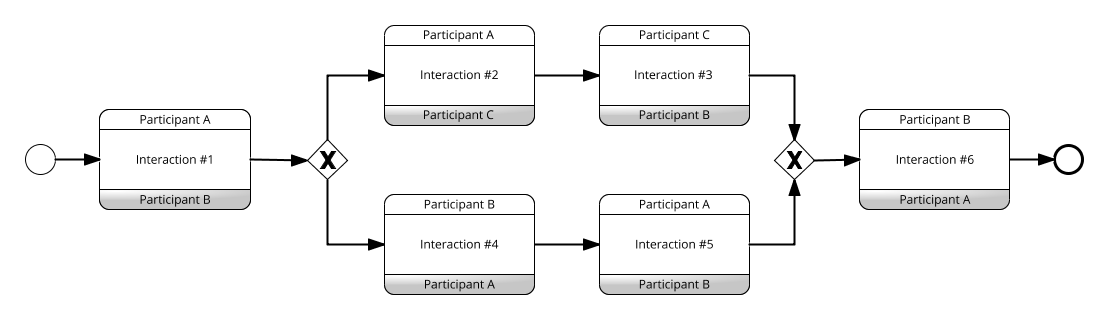
\includegraphics[width=1\textwidth]{src/images/messageFlow.png}
\caption{Message Flow - Sender/Receiver sequence}
\label{fig:messageflow}
\end{figure}

hier noch den algo einfügen bidde...\\
It should be noted, that because of the fact, that the sequence flow is first build without considering the corresponding message flow, it is likly that at some points an additional interaction must be inserted into the model to satisfy the above stated rules of sender-receiver sequences.


\subsection{ComplianceController}
As mentioned in the chapter of ChoreographyController, first a model is genereated and afterwards it is checked, if the interaction sequence specified within the compliance rules, can be applied to the generated model. Until now, the genereated model complies only to the parametric constraints. The logic of specifying and imposing compliance rules is implemented by the \textit{ComplianceController} component.\\

When specifying compliance rules to which the choreography model must comply to, it must be checked, if the imposed rules are consistent with one another. In the context of the four supported patterns (see xx), this applies only to the two order patterns (LeadsTo and Precedes). For instance, consider following set of compliance rules:

\begin{itemize}
\item \textit{CR-1}: P LeadsTo Q
\item \textit{CR-2}: Q LeadsTo S
\item \textit{CR-3}: S Precedes P
\end{itemize}

In this example, the rule \textit{CR-1} in combination with \textit{CR-2} is in conflict with \textit{CR-3}, because \textit{CR-1} and \textit{CR-2} determine, that the involved activities must occur in the order P-Q-S, whereas \textit{CR-3} constrains, that activity S must occur before activity P, which is in violation of the order determined by \textit{CR-1} and \textit{CR-2}. Algorithm \ref{alg:conflictCheck} demonstrates the conflict checking procedure implemented within the complicance controller component. \\

\begin{algorithm}[H]
\DontPrintSemicolon
\SetAlgoLined
\SetKwInOut{Input}{Input}
\SetKwInOut{Output}{Output}
\Input{ 
\begin{itemize}[label={--}]
\item compliance rule $cr$
\item dictionary $orderDependencies$ consisting of Interactions $P$ and their succeeding Interactions $S$
\end{itemize}
}

\SetKwProg{Fn}{Function}{}{}
\Begin{
	\If{$cr$ is order pattern}{
		$p \leftarrow$ preceding interaction of $cr$\;
		$s \leftarrow$ succeeding interaction of $cr$\;
		\eIf{!orderConflictCheck($p, s$)}{
			add $cr$ to $complianceRules$\;
			\eIf{$p \in P$ of $orderDependencies$}{
				add $s$ to succeeding interactions $S$ of $p$
			}{
				add $p$ to $orderDependencies$\;
				add $s$ to succeeding interactions $S$ of $p$ 
			}	
		}{
			add $cr$ to $conflictedRules$\;
		}
	}	
}
\Fn{orderConflictCheck($p, s$)}{
	\eIf{$s \in P$ of $orderDependencies$}{
		\ForEach{$s \in S$ of $p$}{
			\uIf{$s$ == $p$}{
				\Return \textbf{true}
			}\uElseIf{orderConflictCheck($s, p$)}{
				\Return \textbf{true}
			}
		}
	}{
		\Return \textbf{false} 	
	}
}
\caption{Add Compliance Rule}
\label{alg:conflictCheck}
\end{algorithm}

The result of this procdure is a set of conflict free compliance rules, that determine a specific order sequence between the involved interactions.
The specific interactions of the compliance rules are then tried to assign to the exisiting interactions within the before genereated model in a way that it complies to the interaction order and the compliance rules.


\subsection{ChoreographyGenerator}
This component is responsible for the process of deriving the public and private models of each participant from the before generated choreography model.


\section{Translator to BPMN/XML}
